\subsection{Graph-traversal}
  \noindent
  \marginnote{4.3.1.1}There are two ways to traverse a graph:
  \begin{itemize}
  	\item Depth First Search
	  	\subitem In a depth first traversal you first try and go as deep into the graph as possible and once you reach a dead end, you backtrack till you reach a node where one of its neighbours hasn't been visited. It is often called recursively. This is useful for generating and solving mazes.
  	\item Breadth first Search
	  	\subitem In a breadth first traversal, you always try and visit the nodes closest to the previously visited nodes. A queue is often used to keep track of previously visited nodes. This is useful for finding the shortest distance between two nodes for an unweighted graph.
  \end{itemize}
  
  \begin{figure}[H]
  	\includegraphics[scale=0.4]{Undirected-Graph}
  \end{figure}
  
  Using the graph above, we will demonstrate both algorithms:
  
  {\large \textbf{Depth First}}
  
  \begin{table}[H]
  	\begin{tabular}{L{0.8\textwidth} | C{0.1\textwidth} | C{0.1\textwidth}}
  		Explanation & Current Node & Visited Nodes\\\hline
  		Select the node to start from 1. & 1 & \\\hline
  		Mark 1 as visited, choose a node connected to 1 and has not been visited (2) and recursively call the traversal routine to explore from this node. & 1 & 1 \\\hline
  		Mark 2 as visited, choose a node connected to 2 and has not been visited (3) and recursively call the traversal routine to explore from this node. & 2 & 1 2 \\\hline
  		Mark 3 as visited, choose a node connected to 3 and has not been visited (5) and recursively call the traversal routine to explore from this node. & 3 & 1 2 3 \\\hline
  		Mark 5 as visited, choose a node connected to 5 and has not been visited (4) and recursively call the traversal routine to explore from this node. & 5 & 1 2 3 5\\\hline
  		Mark 4 as visited, all nodes connected to 4 have been visited so backtrack until you find a node that has unvisited neighbours. All the nodes have been visited so terminate. & 4 & 1 2 3 5 4\\\hline
  	\end{tabular}
  \end{table}
  
  There are two main ways to define a depth first traversal:
  
  \textbf{Recursively}
  
\begin{verbatim}function Depth-First-Traversal(graph, nodeV)
    mark the nodeV as discovered
    FOR all nodeW adjacent to nodeV in graph
        IF nodeW has not been visited
            Depth-First-Traversal(graph, nodeW)
        ENDIF
    ENDFOR\end{verbatim}
    
  and \textbf{Using a Stack}
  
\begin{verbatim}function Depth-First-Traversal(graph, nodeV)
    let Stack be a stack
    push nodeV onto Stack
    WHILE Stack is not empty
        pop an element from Stack and store it as nodeW
        IF nodeW is not marked as visited:
            mark nodeW as visited
            FOR all nodeX adjacent to nodeW in graph 
                push nodeC onto Stack
            ENDFOR
        ENDIF
    ENDWHILE\end{verbatim}
  
  {\large \textbf{Breadth First}}
  
  \begin{table}[H]
  	\begin{tabular}{L{0.8\textwidth} | C{0.1\textwidth} | C{0.1\textwidth}}
  		Explanation & Current Node & Queue\\\hline
  		Select the node to start from 1. & 1 & 1 \\\hline
  		Dequeue node from the queue (1) as it is about to be fully explored, mark node (1) as fully explored & 1 & \\\hline
  		Add all the nodes that are adjacent to the current node 1 and are not fully explored, and add them to the queue & 1 & 2 3 4 \\\hline
  		Dequeue node from the queue (2) as it is about to be fully explored, mark node (2) as fully explored & 1 & 3 4\\\hline
  		Add all the nodes that are adjacent to the current node 2 and are not fully explored, and add them to the queue & 2 & 3 4 \\\hline
  		Dequeue node from the queue (3) as it is about to be fully explored, mark node (3) as fully explored & 3 & 4 \\\hline
  		Add all the nodes that are adjacent to the current node 3 and are not fully explored, and add them to the queue & 3 & 4 5 \\\hline
  		Dequeue node from the queue (4) as it is about to be fully explored, mark node (4) as fully explored & 4 & 5\\\hline
  		Add all the nodes that are adjacent to the current node 4 and are not fully explored, and add them to the queue & 4 & 5 \\\hline
  		Dequeue node from the queue (5) as it is about to be fully explored, mark node (5) as fully explored & 5 & \\\hline
  		Add all the nodes that are adjacent to the current node 5 and are not fully explored, and add them to the queue & 5 & \\\hline
  		The queue is now empty after checking for adjacent nodes, therefore the algorithm has finished & & \\
  	\end{tabular}
  \end{table}
  
  The pseudo-code for this algorithm is as follows:
  
\begin{verbatim}function Breadth-First-Traversal(graph, root)
    let Queue be a queue
    enqueue root onto Queue
    mark root as considered
    WHILE Queue is not empty
        dequeue an node from Queue and store it as current
        FOR all node adjacent to current in graph
            IF node is not marked as considered:
	            mark node as considered
	            enqueue node to Queue
	        ENDIF
	    ENDFOR
	ENDWHILE\end{verbatim}
  
\subsection{Tree-traversal}
  \noindent
  \marginnote{4.3.2.1}There are three ways of traversing a binary tree:
  \begin{itemize}
  	\item pre-order
	  	\subitem In pre-order, you first visit the root node, you then traverse the left sub-tree, and then traverse the right sub-tree. This method is the same as depth first traversal. (note you visit the root node first)
	  	\subitem This can be used to get a prefix expression (an expression where the operators are before the values to be evaluated) from an expression tree. It can also be used to copy a tree
  	\item in-order
	  	\subitem In in-order, you first traverse the left sub-tree, then you visit the root node, then you traverse the right sub-tree. (note you visit the root node second, in the middle)
	  	\subitem This is used on binary search trees as it returns the values according to the comparator used to set up the binary tree.
  	\item post order
	  	\subitem In post-order, you first traverse the left sub-tree, then traverse the right sub-tree, then visit the root node, This method is the same as the Breadth first traversal. (note you visit the root node last)
	  	\subitem This can be used to get a postfix expression (an expression where the operators are after the values to be evaluated) from an expression tree (converts infix to RPN). It is also used to delete nodes/ emptying a tree (as it deletes from the bottom and works its way up)  
  \end{itemize}
  Whenever I say visit, I mean extract the data from that node. You can see that prefix used for each corresponds to when the root-node is visited, and that you always traverse the left sub-tree before you traverse the right.
  
  The algorithms for each using python would be as follows, which returns a list in the order in which the nodes were traversed.
  
  \begin{python}
def pre_order(root):
	traverse = [root]
	if root.getLeftChild():
		traverse += pre_order(root.getLeftChild())
	if root.getRightChild():
		traverse += pre_order(root.getRightChild())
	return traverse

def in_order(root):
	traverse = []
	if root.getLeftChild():
		traverse += in_order(root.getLeftChild())
	traverse += [root]
	if root.getRightChild():
		traverse += in_order(root.getRightChild())
	return traverse

def post_order(root):
	traverse = []
	if root.getLeftChild():
		traverse += post_order(root.getLeftChild())
	if root.getRightChild():
		traverse += post_order(root.getRightChild())
	traverse += [root]
	return traverse
\end{python}
\subsection{Reverse Polish}
  \noindent
  \marginnote{4.3.3.1} Reverse polish notation is another name for postfix notation which is where the operators are after the values on which they operate. This is in contrast to what we normally use which is infix notation, where the operators are in between the values on which they operate on. An operator is a process within an expression, e.g + - * / etc. an operand is the value that operators work on, a value within the expression. 
  
  A simple way to do this algorithm is to first write out all the operands in the order in which they were originally in the infix expression as that order doesn't change. Then consider step by step, what calculations you would need to do to represent the expression, then for each write it out make sure the operator is after the operands, for example:

5 + ((1 + 2) * 4) − 3

First you add 1 and 2 together (1 2 +), 

then you times that by 4(1 2 + 4 *), then you add 5 to it (remember, 5 appeared first, so it has to be at the beginning of the expression, so 5 1 2 + 4 * +), then you subtract 3 from it (5 1 2 + 4 * + 3 -). The reason that the operands keep their order is due to the algorithm used for the conversion called the shunting yard algorithm, which goes as follows (tokens refer to both operands and operators):
\begin{enumerate}
	\item While there are tokens to be read:
		\subitem Read a token.
		\begin{itemize}
		\item If the token is a number, then push it to the output queue.
		\item If the token is a function token, then push it onto the stack.
		\item If the token is a function argument separator (e.g., a comma):
			\subitem Until the token at the top of the stack is a left parenthesis, pop operators off the stack onto the output queue. If no left parentheses are encountered, either the separator was misplaced or parentheses were mismatched.
		\item If the token is an operator, o1, then:
			\subitem while there is an operator token o2, at the top of the operator stack and either
				o1 is left-associative and its precedence is less than or equal to that of o2, or
				o1 is right associative, and has precedence less than that of o2,
					\subsubitem pop o2 off the operator stack, onto the output queue;
			at the end of iteration push o1 onto the operator stack.
		\item If the token is a left parenthesis (i.e. "("), then push it onto the stack.
		\item If the token is a right parenthesis (i.e. ")"):
			\subitem Until the token at the top of the stack is a left parenthesis, pop operators off the stack onto the output queue.
			\subitem Pop the left parenthesis from the stack, but not onto the output queue.
			\subitem If the token at the top of the stack is a function token, pop it onto the output queue.
			\subitem If the stack runs out without finding a left parenthesis, then there are mismatched parentheses.
		\end{itemize}
	\item When there are no more tokens to read:
		\subitem While there are still operator tokens in the stack:
			\subsubitem If the operator token on the top of the stack is a parenthesis, then there are mismatched parentheses.
			\subsubitem Pop the operator onto the output queue.
\end{enumerate}

You don't need to know the algorithm off by heart, you just need to be able to convert from infix to postfix and vice versa. To convert from postfix to infix (or just evaluate a postfix expression we use the following algorithm):
\begin{enumerate}
	\item While there are input tokens left
		Read the next token from input.
		If the token is a value
			Push it onto the stack.
		Otherwise, the token is an operator (operator here includes both operators and functions).
			It is already known that the operator takes n arguments.
			If there are fewer than n values on the stack
				(Error) The user has not input sufficient values in the expression.
			Else, Pop the top n values from the stack.
			Evaluate the operator, with the values as arguments.
			Push the returned results, if any, back onto the stack.
	\item If there is only one value in the stack
		That value is the result of the calculation.
\end{enumerate}

It may look complicated, but it basically boils down to, read the expression from left to right, where ever you see an operator, evaluate it with the 2 preceding values, and replace them with the new value, for example,
consider 5 + ((1 + 2) * 4) − 3 was converted to its postfix notation
5 1 2 + 4 * + 3 -
The steps to evaluate it would be (left shows conversion to infix, right shows evaluation, both go through the same algorithm, you just decide whether or not to simplify the expression on the way down):

\begin{table}[H]
	\begin{tabular}{cc}
		5 (1+2) 4 * + 3 - & 5 3 4 * + 3 - \\
		5 ((1+2)*4) + 3 - & 5 12 + 3 - \\
		5 + ((1+2)*4) 3 - & 17 3 - \\
		5 + ((1+2)*4) - 3 & 14 \\
	\end{tabular}
\end{table}

The main upside of postfix notation is that it eliminates the need for brackets within the expression, as the expression is evaluated from left to right, with operators acting on previous two values. It also means that expressions can easily be evaluated via the use of a stack. It is also used in interpreters which are based on a stack, such as with Postscript (a programming language used to describe a page's text and graphical content) and bytecode.


\subsection{Searching Algorithms}
  \noindent
	  \marginnote{4.3.4.1}In a linear search, you just check each item in a list sequentially to see if the item you are looking for is in the list. This approach isn't especially efficient, but must be used if you are dealing with a list that has no inherent order to it. It has a time complexity of $O(n)$. Sample python code would be as follows:
	  
\begin{python}
def linear_search(lis, item):
	for ele in lis:
		if ele == item:
			return True
	return False
\end{python}

  \noindent
  \marginnote{4.3.4.2}A binary search can be used on a list that has some sort of logical ordering. It works off of the premise that in an ordered list, if you were to play a game of higher or lower, always choosing the middle of the remaining list, will allow you to eliminate half of the remaining list, allowing you to quickly deduce where (or if) an element is in the list. It has a time complexity of $O(\lg(n))$. An algorithm in python would be as follows:

\begin{python}
def binary_search(lis, item):
	low_pointer = 0
	high_pointer = len(lis)-1
	while low_pointer<=high_pointer:
		mid_pointer = (low_pointer + high_pointer)//2
		if item < lis[mid_pointer]:
			high_pointer = mid_pointer-1
		if item > lis[mid_pointer]:
			low_pointer = mid_pointer+1
		if item == lis[mid_pointer]:
			return True
	return False
\end{python}

  \noindent
  \marginnote{4.3.4.3}A Binary Tree is often used in programs where data is very dynamic, data is constantly being added and taken away from the system. To search through a binary tree is similar to searching an ordered list, except instead you are searching through a tree, thus you must traverse the tree and look at the items in each node. It has a time complexity of $O(\lg(n))$. Example python code would be:
  
\begin{python}
def binary_search(root,item):
	current_node = root
	while True:
		if current_node.getLabel() > item:
			current_node = current_node.getLeftChild()
		elif current_node.getLabel() < item:
			current_node = current_node.getRightChild()
		else:
			return True
		if current_node == None:
			return False
\end{python} 
\subsection{Sorting Algorithms}
  \noindent
  \marginnote{4.3.5.1}The bubble sort is a simple way of ordering a list. The algorithm can easily be described as follows: Until the list is ordered, go along the list comparing each element to its next element, if the current element is greater than the next element, swap the elements, else continue.
\begin{python}
def bubblesort(lis):
	for i in range(len(lis)):
		for j in range(len(lis)-1):
			if lis[j] > lis[j + 1]:
				temp = lis[j+1]
				lis[j+1]=lis[j]
				lis[j]=temp
	return lis
\end{python}

this algorithm can be written in a more sophisticated manner (so that it ends if no swaps occur, as this implies it is sorted, thus not going through unneeded iterations) as follows:
\begin{python}
def bubblesort(lis):
	while True:
		completedFlag = True
			for j in range(len(lis)-1):
				if lis[j] > lis[j + 1]:
					temp = lis[j+1]
					lis[j+1]=lis[j]
					lis[j]=temp
					completedFlag = False
		if completedFlag:
			return lis
					
\end{python}

A quick trace through the algorithm after every while loop for the list [3,5,1,6,2,4,7,8] would be as follows:

\begin{table}
	\begin{tabular}{C{0.05\textwidth} | C{0.05\textwidth} | C{0.05\textwidth} | C{0.05\textwidth} | C{0.05\textwidth} | C{0.05\textwidth} | C{0.05\textwidth} | C{0.05\textwidth} | C{0.05\textwidth} | C{0.3\textwidth}}
		Pass & list[0] & list[1] & list[2] & list[3] & list[4] & list[5] & list[6] & list[7] & completedFlag \\\hline
		0 & 3 & 5 & 1 & 6 & 2 & 4 & 7 & 8 & True (no passes have been done yet) \\\hline
		1 & 3 & 1 & 5 & 2 & 4 & 6 & 7 & 8 & False \\\hline
		2 & 1 & 3 & 2 & 4 & 5 & 6 & 7 & 8 & False \\\hline
		3 & 1 & 2 & 3 & 4 & 5 & 6 & 7 & 8 & False \\\hline
		4 & 1 & 2 & 3 & 4 & 5 & 6 & 7 & 8 & True \\
	\end{tabular}
\end{table}


The bubble sort algorithm is one of the least efficient sorting algorithms and has a time complexity of $O(n^2)$, and attempts should be made to try and use better sorting algorithms.

  \noindent
  \marginnote{4.3.5.2}Merge Sort is an algorithm which works by first splitting the original list into 2 halves, merge sorting each of the halves, then merging the two half lists so that it creates an ordered list, this is an example of a divide and conquer strategy to problem solving. As you can tell, this is a recursive sort, and has the base case of a single element, because a single element is already sorted. Python code for the merge sort (and a separate function for the merging) are as follows:

\begin{python}
def mergesort(lis):
	if len(lis)==1:
		return lis
	else:
		lis1 = mergesort(lis[0:len(lis)//2])
		lis2 = mergesort(lis[len(lis)//2:len(lis)])
		return merge(lis1,lis2)

def merge(lis1,lis2):
	res = []
	while (len(lis1)!=0 and len(lis2)!=0):
		if lis1[0] < lis2[0]:
			res.append(lis1[0])
			del lis1[0]
		else:
			res.append(lis2[0])
			del lis2[0]
	while len(lis1)!=0:
		res.append(lis1[0])
		del lis1[0]
	while len(lis2)!=0:
		res.append(lis2[0])
		del lis2[0]
	return res
\end{python}

This is a much more efficient sorting algorithm than the bubble sort and has time complexity $O(n\lg(n))$. A brief trace of the algorithm for the list [3,5,1,6,2,4,7,8] would be as follows:

\begin{enumerate}
	\item [3,5,1,6,2,4,7,8]
	\item [3,5,1,6] [2,4,7,8]
	\item [3,5] [1,6] [2,4] [7,8]
	\item [3] [5] [1] [6] [2] [4] [7] [8]
	\item [3,5] [1,6] [2,4] [7,8]
	\item [1,3,5,6] [2,4,7,8]
	\item [1,2,3,4,5,6,7,8]
\end{enumerate}

\subsection{Optimisation Algorithms}
  \noindent
  \marginnote{4.3.6.1}Dijkstra's shortest path algorithm is an algorithm used to find the shortest path between two nodes in a graph (mainly weighted). This algorithm has several useful applications:
  \begin{itemize}
  	\item Geographic Information systems (GIS)
	  	\subitem Satellite Navigation
	  	\subitem Mapping software
	\item Telephone and Computer Network Planning
	\item Network Routing/ Packet Switching
	\item Logistics and Scheduling
  \end{itemize}
  
  Dijkstra's Algorithm goes as follows:
  \begin{enumerate}
  	\item Give all of the existing nodes a value corresponding to their current perceived distance according to the following rules: set it to zero for our initial node and to infinity for all other nodes.
  	\item Set the initial node as current. Mark all other nodes unvisited. Create a set of all the unvisited nodes called the unvisited set.
  	\item For the current node, consider all of its unvisited neighbours and calculate their tentative distances. Compare the newly calculated perceived distance to the current assigned value and assign the smaller one. For example, if the current node A is marked with a distance of 6, and the edge connecting it with a neighbour B has length 2, then the distance to B (through A) will be 6 + 2 = 8. If B was previously marked with a distance greater than 8 then change it to 8. Otherwise, keep the current value.
  	\item When we are done considering all of the neighbours of the current node, mark the current node as visited and remove it from the unvisited set. A visited node will never be checked again.
  	\item If the destination node has been marked visited (when planning a route between two specific nodes) or if the smallest perceived distance among the nodes in the unvisited set is infinity (when planning a complete traversal; occurs when there is no connection between the initial node and remaining unvisited nodes), then stop. The algorithm has finished.
  	\item Otherwise, select the unvisited node that is marked with the smallest tentative distance, set it as the new "current node", and go back to step 3.
  \end{enumerate}
  
  For the following graph, the Trace of the algorithm from node A to node K would be (the subscript next to numbers shows the node to which the shortest path would come from):
  \begin{center}
  	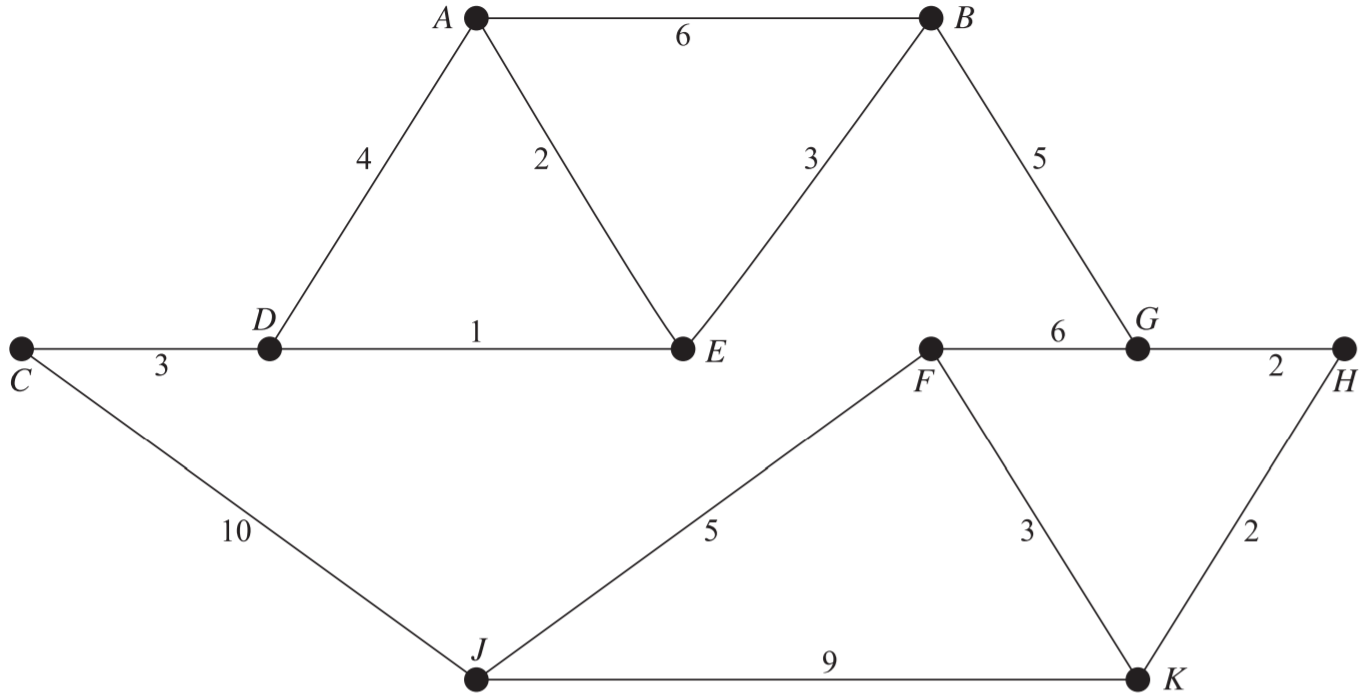
\includegraphics[scale=0.4]{Dijkstra-Graph}
  \end{center}
  
  \begin{table}[H]
  	\begin{tabular}{c c c c c c c c c c c c}
  		Step & Vertex & A & B & C & D & E & F & G & H & J & K \\ 
  		0 & A & $0_A$ & $\infty_A$ & $\infty_A$ & $\infty_A$ & $\infty_A$ & $\infty_A$ & $\infty_A$ & $\infty_A$ & $\infty_A$ & $\infty_A$  \\
  		1 & A & $0_A$ & $6_A$ & $\infty_A$ & $4_A$ & $2_A$ & $\infty_A$ & $\infty_A$ & $\infty_A$ & $\infty_A$ & $\infty_A$  \\
  		2 & E & $0_A$ & $5_E$ & $\infty_A$ & $3_E$ & $2_A$  & $\infty_A$ & $\infty_A$ & $\infty_A$ & $\infty_A$ & $\infty_A$  \\
  		3 & D & $0_A$ & $5_E$ & $6_D$ & $3_E$ & $2_A$  & $\infty_A$ & $\infty_A$ &  $\infty_A$ & $\infty_A$ & $\infty_A$ \\
  		4 & B & $0_A$ & $5_E$ & $6_D$ & $3_E$ & $2_A$  & $\infty_A$ & $10_B$ &  $\infty_A$ & $\infty_A$ & $\infty_A$ \\
  		5 & C & $0_A$ & $5_E$ & $6_D$ & $3_E$ & $2_A$  & $\infty_A$ & $10_B$ & $\infty_A$ & $16_C$ & $\infty_A$ \\
  		6 & G & $0_A$ & $5_E$ & $6_D$ & $3_E$ & $2_A$  & $16_G$ & $10_B$ & $12_G$ & $16_C$ & $\infty_A$ \\
  		7 & H & $0_A$ & $5_E$ & $6_D$ & $3_E$ & $2_A$  & $16_G$ & $10_B$ & $12_G$ & $16_C$ & $14_H$ \\
  		8 & K & $0_A$ & $5_E$ & $6_D$ & $3_E$ & $2_A$  & $16_G$ & $10_B$ & $12_G$ & $16_C$ & $14_H$ \\
  	\end{tabular}
  \end{table}
  
  We can use this to trace back and find that the shortest route is A-E-B-G-H-K
  